\documentclass[,a4paper,12pt,french]{article}

\usepackage{Styletest}

\usepackage[d]{esvect}

\usepackage{minted}
\usemintedstyle{rainbow_dash} % Styles sympa: default,manni,monokai,pastie,native,igor,lovelace,rainbow_dash,inkpot,
\setminted{xleftmargin=\parindent,linenos,
    gobble=0,
    breaklines=true,
    breakafter=,,
    numbersep=8pt}

\usepackage{listings}

\tcbuselibrary{minted,skins,xparse}

\DeclareTCBListing{mintedbox}{O{}m!O{}}{%
	frame style={fill},
	boxrule=1pt,
rounded corners,
  breakable=true,
  listing engine=minted,
  listing only,
  minted language=#2,
  minted style=rainbow_dash,
  minted options={%
    linenos,
    gobble=0,
    breaklines=true,
    breakafter=,,
    numbersep=8pt,
    #1},
  boxsep=0pt,
  left skip=0pt,
  right skip=0pt,
  left=25pt,
  right=0pt,
  top=3pt,
  bottom=3pt,
  arc=5pt,
  leftrule=0pt,
  rightrule=0pt,
  bottomrule=2pt,
  toprule=2pt,
  colback=orange!5,
  colframe=orange!70,
  enhanced,
  overlay={%
    \begin{tcbclipinterior}
    \fill[orange!20!white] (frame.south west) rectangle ([xshift=20pt]frame.north west);
    \end{tcbclipinterior}},
  #3}



\definecolor{couleurNombres}{rgb}{0.35,0.09,0.73}
\definecolor{couleurFonctions}{rgb}{1.00,0.50,0.00}
\definecolor{keyword}{rgb}{0.17,0.36,0.80}

\makeatletter
% This macro makes the style commands
% #1 -- the name of the command, 
% #2 -- the styling code
\def\makeHighlightCommand#1#2{%
    \gdef#1##1{%
        \testkern{##1}% Check if ##1 starts with \kern, if so just output it
        {% else do this code
            \edef\testa{\the\lst@token}% The actual thing to be typeset is in \lst@token
            \def\testb{:}%
            \ifx\testa\testb % Test whether lst@token is just : 
                :% if so print the colon
                 % we're done now but for some reason \lst@currstyle (which is what 
                 % contains this function) doesn't go out of scope correctly.
                \global\let\lst@currstyle\relax % So we explicitly set it to \relax
            \else
                #2% Use the styling code
            \fi
        }%
    }%  
}  

% Tests if the first argument starts with \kern, 
% if so, just outputs its first argument, otherwise just outputs its second argument    
\def\testkern#1{\testkern@#1\relax\nil}
\def\testkern@#1#2\nil{\ifx#1\kern #1#2\expandafter\@gobble\fi}

% Uses listing's internal method to output a sequence of letters
% makes them super far apart like all the other letters
\def\lsttt#1{%
    \bgroup
    \let\lst@currstyle\relax
    \lsttt@#1.
    \egroup
}
\def\lsttt@#1{\ifx#1.\else\lst@length=1\lst@token{#1}\lst@Output\expandafter\lsttt@\fi}
\makeatother
\lstset{
  language=python,
  xleftmargin=\parindent,
  numbersep=8pt,
  basicstyle=\ttfamily,
  columns=fullflexible,
  keepspaces=true,
  numbers=left,
  numberstyle=\tiny,
  keywordstyle=[1]{\color{keyword}\bfseries},
  keywordstyle=[2]{\color{keyword}},
  emphstyle=\color[rgb]{1.00,0.50,0.00}\bfseries,
  %identifierstyle=\color{gray},
  stringstyle=\color[rgb]{0.639,0.082,0.082}\ttfamily,
  moredelim={*[is][\functionHighlight]{def\ }{(}},
  otherkeywords={+,-,*,/,=,>,<},
  morekeywords=[2]{+,-,*,/,=,>,<},
  literate=%
   *{0}{{{\color{couleurNombres}\bfseries 0}}}1
    {1}{{{\color{couleurNombres}\bfseries 1}}}1
    {2}{{{\color{couleurNombres}\bfseries 2}}}1
    {3}{{{\color{couleurNombres}\bfseries 3}}}1
    {4}{{{\color{couleurNombres}\bfseries 4}}}1
    {5}{{{\color{couleurNombres}\bfseries 5}}}1
    {6}{{{\color{couleurNombres}\bfseries 6}}}1
    {7}{{{\color{couleurNombres}\bfseries 7}}}1
    {8}{{{\color{couleurNombres}\bfseries 8}}}1
    {9}{{{\color{couleurNombres}\bfseries 9}}}1
}

\makeHighlightCommand\functionHighlight{{\color{keyword}\bfseries\lsttt{def}}{{\bfseries\color{couleurFonctions}#1}}(}


% Début du document
%%%%%%%%%%%%%%%%%%%
\begin{document}

\titre{Fonctions - Exercices}
\begin{thm}[Quelques test] \
\begin{centrer}
\begin{tikzpicture}[scale=\echellepgf]
\begin{axis}[
styleglobal,
width=0.8*\echellepgfinv*\linewidth,
xmin=-0.5, xmax= 8.5,
ymin=-2.5, ymax=3.5,
xtick distance=1,
ytick distance=1,
minor x tick num=1,
minor y tick num=1,
]
\addplot[styleplot,domain=(0:8)] plot {0.5*x-1.5)} node[pos=0.75,above] {$\mathscr C_f$} \pointsextremites;
\addplot[styleplot,color=DarkRed,densely dashed,domain=(0:8)] plot coordinates{(0,-2) (1,-1) (2,2) (3,3) (5,1) (6,0) (8,-2)} node[pos=0.6,above right] {$\mathscr C_g$};
\addplot[styleplot,densely dotted,color=DarkGreen,domain=(0:8)] plot coordinates{(0,3) (2,2) (3,0) (4,-2) (6,0) (7,2) (8,3)} node[pos=0.1,above right] {$\mathscr C_h$};
\end{axis}
\end{tikzpicture}
\end{centrer}

\ \newline

\compo[0.5]
{
\begin{centrer}

Sans hauteurproptick

\begin{tikzpicture}[scale=\echellepgf]
\begin{axis}[
styleglobal,
width=0.8*\echellepgfinv*\linewidth,
xmin=0, xmax= 25,
ymin=-12, ymax=16,
xtick distance=2,
ytick distance=4,
minor x tick num=1,
minor y tick num=0,
ylabel={Température ($^{\circ}$C)},
xlabel={Temps (h)},
label style={font=\normalsize},
%yscale=0.5,
]
\addplot[styleplot] plot coordinates {(0,10) (1,6) (2,2) (5,-4) (6,-8) (8,-10) (10,-8) (13,2) (15,8) (16,12) (18,14) (20,2) (24,-4)};
\end{axis}
\end{tikzpicture}
\end{centrer}
}
{
\begin{centrer}

Avec hauteurproptick

\begin{tikzpicture}[scale=\echellepgf]
\begin{axis}[
styleglobal,
hauteurproptick,
width=0.8*\echellepgfinv*\linewidth,
xmin=0, xmax= 26,
ymin=-12, ymax=16,
xtick distance=2,
ytick distance=4,
minor x tick num=1,
minor y tick num=0,
ylabel={Température ($^{\circ}$C)},
xlabel={Temps (h)},
xlabel near ticks,
ylabel near ticks,
xlabel shift={5mm},
%x label style={at={(ticklabel cs:0.5)},anchor=near ticklabel},
%y label style={at={(ticklabel cs:0.5)},rotate=90,anchor=near ticklabel},
label style={font=\normalsize},
%y post scale=0.5,
%xtick style={/pgfplots/major tick length=1/\pgfkeysvalueof{/pgfplots/yscale}*0.15cm,/pgfplots/minor tick length=1/\pgfkeysvalueof{/pgfplots/yscale}*0.1cm},
]
\addplot[styleplot] plot coordinates {(0,10) (1,6) (2,2) (5,-4) (6,-8) (8,-10) (10,-8) (13,2) (15,8) (16,12) (18,14) (20,2) (24,-4)};
\end{axis}
\end{tikzpicture}
\end{centrer}
}

\begin{tikzpicture}
\tkzTabInit[lgt=1.5]{$x$ /1, $f'(x)$/1, $f(x)$ / 2}{$- \infty$, $0$, $+ \infty$}

\tkzTabLine{,-,z,+}

\tkzTabVar{+/$+ \infty$, -/ -2, +/ $+\infty$}

\tkzTabVal 1 2 {0.5} {} 0;
\tkzTabVal 2 3 {0.5} {} 0;

\end{tikzpicture}

BLABLABLA teeeest

\end{thm}

\begin{centrer}
\begin{tikzpicture}[]
\tkzTabInit[lgt=1.5]{$x$ /1, $f'(x)$/1, $f(x)$ / 2}{$- \infty$, $0$, $+ \infty$}

\tkzTabLine{,-,z,+}

\tkzTabVar{+/$+ \infty$, -/ -2, +/ $+\infty$}

\tkzTabVal 1 2 {0.5} {} 0;
\tkzTabVal 2 3 {0.5} {} 0;

\end{tikzpicture}
\end{centrer}

$$\vec u \vec{AB} \vecc u \vecc{AB}$$

$$\vv u \vv{AB}$$

$\mathbb {NZDQRCUKEP}$

$\mathds {NZDQRCUKEP}$

Problème: minted et listing utilisent un package fragile qui ne peut pas s'encapsuler: compo ne fonctionne pas mais on peut le reproduire à la main:

\begin{minipage}{0.49\linewidth}

\begin{minted}{python}
def zero(f,a,b,seuil):
    while (b-a)/2>seuil:
        c=(a+b)/2
        if f(c)==0:
            return(c)
        if f(a)*f(c)>0:
            a=c
        else:
            b=c
    return((a+b)/2)

def f(x):
    return(x**2-2)

\end{minted}
\center{Minted}
\end{minipage}\hfill\begin{minipage}{0.49\linewidth}
\begin{lstlisting}
def zero(f,a,b,seuil):
    while (b-a)/2>seuil:
        c=(a+b)/2
        if f(c)==0:
            return(c)
        if f(a)*f(c)>0:
            a=c
        else:
            b=c
    return((a+b)/2)

def f(x):
    return(x**2-2)

\end{lstlisting}
\center{Listing avec style minted}
\end{minipage} \par

Ceci est un test: \mintinline{python}|def zero(f,a,b,seuil):| permet de \lipsum[1]

\begin{mintedbox}{python}
def zero(f,a,b,seuil):
    while (b-a)/2>seuil:
        c=(a+b)/2
        if f(c)==0:
            return(c)
        if f(a)*f(c)>0:
            a=c
        else:
            b=c
    return((a+b)/2)

def f(x):
    return(x**2-2)
\end{mintedbox}

Ceci est un test

\end{document}
